\section{Partition function}

Theories with an action can be quantized using a path integral.
The partition function in Euclidean signature is defined as
% \footnote{
% Wick rotation analytically continues time to imaginary (Euclidean) time, $t\rightarrow -i t_E$,
% then the oscillatory exponential becomes decaying. }
% the same as the canonical partition function in statistical mechanics. }
\begin{equation}
 Z = \int D\phi \, e^{-S[\phi]},
\end{equation}
which is an infinite-dimensional integral, 
over all possible field configurations (represented by the measure $D\phi$) on all of spacetime.


For $\mathcal{N}=2^*$ on $S^4$ and its limiting cases $\mathcal{N}=4$ (massless hypermultiplet) and pure $\mathcal{N}=2$ (infinitely-heavy hypermultiplet that is integrated out), 
there is one localization locus.
It is the moduli space of Coulomb vacua, 
parametrized by the vacuum expectation value of a scalar of the vector multiplet:
\begin{equation}\label{vevScalar}
 \braket{\Phi_0} = \text{diag}(a_1, \ldots, a_N), 
\end{equation}
where $a_i$ are real numbers.
The Coulomb phase of the theory 
is a consequence of the spontaneous symmetry breaking of the bosonic quartic potential $\sim [\Phi_I, \Phi_J]^2$,
that breaks the original gauge group $U(N)$ to $U(1)^{N}$.

The result for the localized partition function is of the form:
\begin{equation}\label{Zmatrixmodel}
 Z=\int \; d^N a \, \prod_{i<j} (a_i-a_j)^2 \; Z_\text{1-loop}(a)\; \left|Z_\text{inst}(a)\right|^2\; e^{- \frac{8\pi^2 N}{\lambda} \sum_k a_k^2}.
\end{equation}
The classical action comes from the curvature coupling of the scalars in \eqref{SS4}.

The 1-loop correction, for the different theories are
\begin{eqnarray}
 \text{$\mathcal{N}=2^*$ SYM:}  & & Z_\text{1-loop} = \prod_{i<j} \dfrac{H^2(a_i-a_j)}{H(a_i-a_j-MR) H(a_i-a_j+MR)}\\
 \text{$\mathcal{N}=2$ SYM:}  & & Z_\text{1-loop} = \prod_{i<j} H^2(a_i-a_j) \\
 \text{$\mathcal{N}=4$ SYM:}  & & Z_\text{1-loop} = 1
\end{eqnarray}
where 
\begin{equation}
 H(x) \equiv \prod_{n=1}^{\infty}\left(1+\dfrac{x^2}{n^2}\right)^n e^{-\frac{x^2}{n}}.
\end{equation}
% This function is $1$ at the origin and vanishes very fast away from it.
We used the 't Hooft coupling $\lambda = g_{YM}^2 N$,
and $R$ is again the radius of the hypersphere.


The instanton partition function is the generating function of instantons of topological charge $k$:
\begin{equation}
 Z_\text{inst} = \sum_{k=0}^\infty (e^{i 2\pi\tau})^k Z_k,
\end{equation}
where $Z_0 = 1$ and 
\begin{equation}
\tau = i \frac{4\pi}{g_\text{YM}^2} + \frac{\theta}{2\pi} 
\end{equation}
is the complexified Yang-Mills coupling\footnote{
The instanton action is the pure Yang-Mills action with an additional topological term.
For an instanton of charge $k$, the action is given by:
\[
S_\text{YM} (k)=
    -\frac{1}{2 g_\text{YM}^2} \text{tr} \int d^4 x \sqrt{g} F_{\mu\nu} F^{\mu\nu}
    -i \frac{\theta}{8\pi^2} \text{tr} \int F \wedge F 
    = \left( \frac{8\pi^2}{g_\text{YM}^2} - i \theta \right) k
    = - i 2 \pi \tau \, k. 
\]
% This action breaks CP symmetry.
% In QCD, there is no experimental evidence of CP violation, hence $\theta$ must be very small,
% and it is a considered a fine-tuning problem called the strong CP problem.
}.
% Instantons are tunnelling events in Minkowski signature
% In QCD, the groundstate, called the $\theta$-vacuum, is considered the superposition of all vacua. }.

For the $\mathcal{N}=4$ case, $Z_\text{inst} = 1$, \cite{Okuda:2010ke}.
For the $\mathcal{N}=2$ cases, it is non-trivial, \cite{Nekrasov:2002qd}.
However, the regime of interest is the large $N$ limit:
\begin{equation}\label{largeNlimit}
 N\rightarrow \infty \quad \text{and} \quad \lambda = g_\text{YM}^2 N \quad \text{is kept finite},
\end{equation}
then the expansion parameter becomes
$$e^{i 2\pi\tau}=e^{-\frac{8\pi^2 N}{\lambda} + i \theta},$$
hence the instanton contributions are expected to be exponentially suppressed. 
This is checked in \cite{Russo:2013kea}.


% 
% for a single instanton in $\mathcal{N}=2^*$
% \begin{equation}
%  Z_\text{1-inst} = - e^{-\frac{8\pi^2 N}{\lambda} + i \theta} (M R)^2 
% 		  \sum_{l=1}^N \prod_{j\neq l}^N \dfrac{ (a_l-a_j +i)^2 - (MR)^2}{(a_l-a_j) (a_l-a_j+2i)}
% \end{equation}
% Integral representation
% \begin{equation}
%  Z_\text{1-inst} = e^{-\frac{8\pi^2 N}{\lambda} + i \theta} \dfrac{2 (M R)^2}{(M R)^2+1} 
% 		  \int \frac{dz}{2\pi} \prod_{j=1}^N \dfrac{(z-a_j)^2 - (MR)^2}{(z-a_j)^2+1}
% \end{equation}









\section{Large-$N$ matrix model}

The localized partition function \eqref{Zmatrixmodel} is a matrix model.
% Therefore, it is convenient to think of it as an analogous statistical model, as we shall see.
For the $\mathcal{N}=4$ case, the model is particularly simple, 
it is the well-known Gaussian unitary ensemble (GUE) in the random matrix theory.
The product of the eigenvalue differences is the Vandermonde determinant squared, 
which is essentially the Jacobian factor after diagonalizing the Hermitean matrix in \eqref{vevScalar}.
Writing it in terms of the effective action:
\begin{equation}\label{eq:ZGUE}
 Z_\text{GUE} = \int \; d^N a \;  e^{- S[a]}, 
 \quad S[a]=- \sum_{i\neq j}^N \log(|a_i-a_j|) + \frac{8\pi^2 N}{\lambda} \sum^N_k a_k^2
\end{equation}
we see that the Vandermonde determinant gives the 2d Coulomb potential.
This partition function is indeed identified with that of a 2d Coulomb gas confined on a line,
with the repulsive electrostatic force and an attractive harmonic force \cite{Dyson:1962es}.


% Exact methods exist, 
% such as the orthogonal polynomial method, 
% to solve the spectral distribution.
% These allow physicists to compute observables exactly for $\mathcal{N}=4$ (cite Genis).

For $\mathcal{N}=2^*$, the matrix model is highly non-trivial, 
but we can solve it systematically in the large $N$ limit,
where the saddle-point approximation and the continuous approximation in principle apply.
The only relevant quantity to compute then is the distribution of the eigenvalues:
\begin{equation} \label{def:rho}
\rho(x) = \dfrac{1}{N} \, \sum_{i=1}^N \delta(x-a_i) .
\end{equation}
It must have a compact support, i.e. $\rho(\pm \mu) = 0$,
where the endpoint $\mu$ determines the scale of the spontaneous symmetry breaking.
By definition, it is also unit-normalized:
\begin{equation}
 \int_{-\mu}^\mu dx\, \rho(x) = 1.
\end{equation}


The saddle-point equation, from extremizing the effective action \eqref{eq:ZGUE} in terms of \eqref{def:rho}, 
is a singular (principal value) integral equation:
\begin{equation} \label{saddlepointEq}
 \dfrac{\delta S [\rho]}{\delta \rho(x)} = 0 \quad
 \Rightarrow \quad
 \fint_{-\mu}^\mu dy \, K(x-y) \rho(y) = \dfrac{8\pi^2}{\lambda}x.
\end{equation}
The singular kernel for the GUE case is just the Hilbert kernel\footnote{
The name is in relation with the Hilbert transform. 
It is also known as Cauchy kernel in the literature.},
that is 
\begin{equation}
 K_\text{Hilbert}(x)=\dfrac{1}{x}.
\end{equation}
In the Coulomb gas picture, the saddle-point equation determines the equilibrium distribution due to the force balance.
The result is the well-known Wigner's semicircle distribution
\begin{equation}\label{semicircle}
 \rho(x) = \dfrac{2}{\pi \mu^2} \sqrt{\mu^2-x^2}, 
 \quad \mu = \dfrac{\sqrt{\lambda}}{2\pi},
\end{equation}
shown in figure \ref{fig:semicircle}.


\begin{figure}[t]
\begin{center}
 \centerline{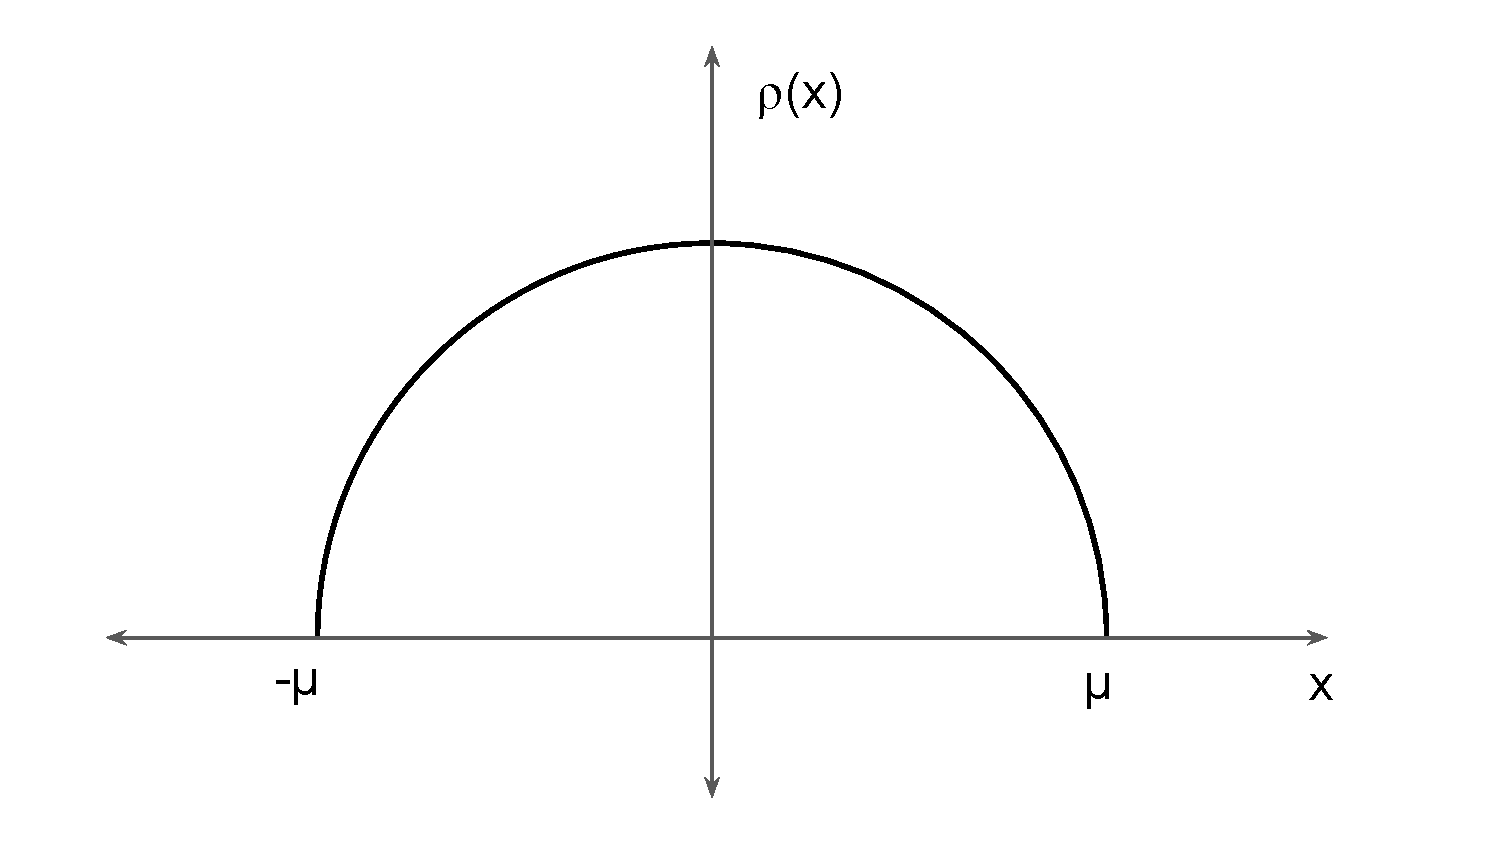
\includegraphics[width=0.8\textwidth]{Images/semicircle.pdf}}
 \caption{\label{fig:semicircle} Wigner's semicircle distribution, solution to the Gaussian unitary ensemble (GUE).}
\end{center}
\end{figure}

For the $\mathcal{N}=2^*$ SYM, the kernel is
\begin{equation}
 K(x)=\dfrac{1}{x}-\mathcal{K}(x)+\dfrac{1}{2}\,\mathcal{K}(x+MR)+\dfrac{1}{2}\,\mathcal{K}(x-MR),
\end{equation}
where 
\begin{equation}
 \mathcal{K}(x) \equiv -\dfrac{H'(x)}{H(x)} 
                = 2x\sum_{n=1}^{\infty} \left(\dfrac{1}{n}-\dfrac{n}{n^2+x^2} \right),
\end{equation}
and much more interesting features show up in the saddle-point solution, as shown in figure \ref{fig:phaseDiagram}.
Let us briefly review these results.


In the strong-coupling regime, the bulk of the distribution is also a semicircle but with a rescaled endpoint:
\begin{equation}\label{semicircleN=2*}
 \rho(x) = \dfrac{2}{\pi \mu^2} \sqrt{\mu^2-x^2}, 
 \quad
 \mu=\dfrac{\sqrt{\lambda (1+(MR)^2)}}{2\pi},
 \quad (\lambda \rightarrow \infty).
\end{equation}
This is due to the fact that the kernel is approximately a Hilbert kernel \cite{Buchel:2013id}:
\begin{equation} \label{Kapprox}
 K(x) \approx \dfrac{1+(MR)^2}{x}, \quad (\lambda \rightarrow \infty).
\end{equation}
Close to the edge-points, this approximation no longer holds,
and it was the goal of Paper I to find the endpoint distribution in the strong coupling regime.

We computed the endpoint distribution exactly using the so-called Wiener-Hopf method, 
which is essentially the Fourier transform of the convolution integral in \eqref{saddlepointEq} in a semi-infinite interval 
(zero being at the endpoint),
that relies on a certain factorization of the kernel.

The distribution exhibits oscillatory behavior with a period proportional to the scale $M R$. 
In the decompactification limit $MR\rightarrow \infty$ (but $\mu\gg MR$ because we remain in the strong coupling limit), 
the peaks of the oscillation diverge, see figure \ref{fig:phaseDiagram}.
The analytical endpoint distribution at strictly infinite coupling and flat space, with $\xi\equiv\mu-x$, is summarized below:
\begin{equation}
 \rho(\xi )= \frac{2^{3/2}}{\pi \mu^{3/2}}
% \frac{\sqrt{2 M R}}{\pi \mu^{3/2}}
 \begin{cases}
   MR \sqrt{\xi}, 
   &\quad (\xi \sim 1)\\
   \dfrac{\sqrt{M R}}{2}\sum_{k=0}^{\left[\frac{\xi }{MR}\right]}
             \left(\left\{\frac{\xi }{MR}\right\} + k\right)^{-1/2}
   &\quad (\xi \sim M R),
 \end{cases}
\end{equation}
where $[\cdot]$ and $\{\cdot\}$ denote the integer and the fractional part, respectively, 
and $\mu=MR\sqrt{\lambda}/(2\pi)$, from \eqref{semicircleN=2*}.

Physically, the cusps appear due to a resonance phenomena 
\begin{equation}
m_{ij} = |a_i-a_j \pm MR| \approx 0
\end{equation}
of very light states in the hypermultiplet sector.
Similar features were already observed for finite couplings in the flat space limit \cite{Russo:2013qaa},
and it was numerically shown that there are infinite-many critical couplings defined by 
\begin{equation}
 \mu = g(\lambda_c^{(n)}) M R, \quad g(\lambda_c^{(n)}) = \dfrac{n}{2}, \quad n=1,\ldots
\end{equation}
This means there are infinitely many phase transitions, where the phases are distinguished by the number of cusps of the distribution,
and the coupling $\lambda$ is the order parameter.
At strong coupling, the critical behavior persists and matches with the one obtained from the decompactification limit, 
hence these two limits commute \cite{Zarembo:2014ooa}.




\begin{figure}[t]
\begin{center}
 \centerline{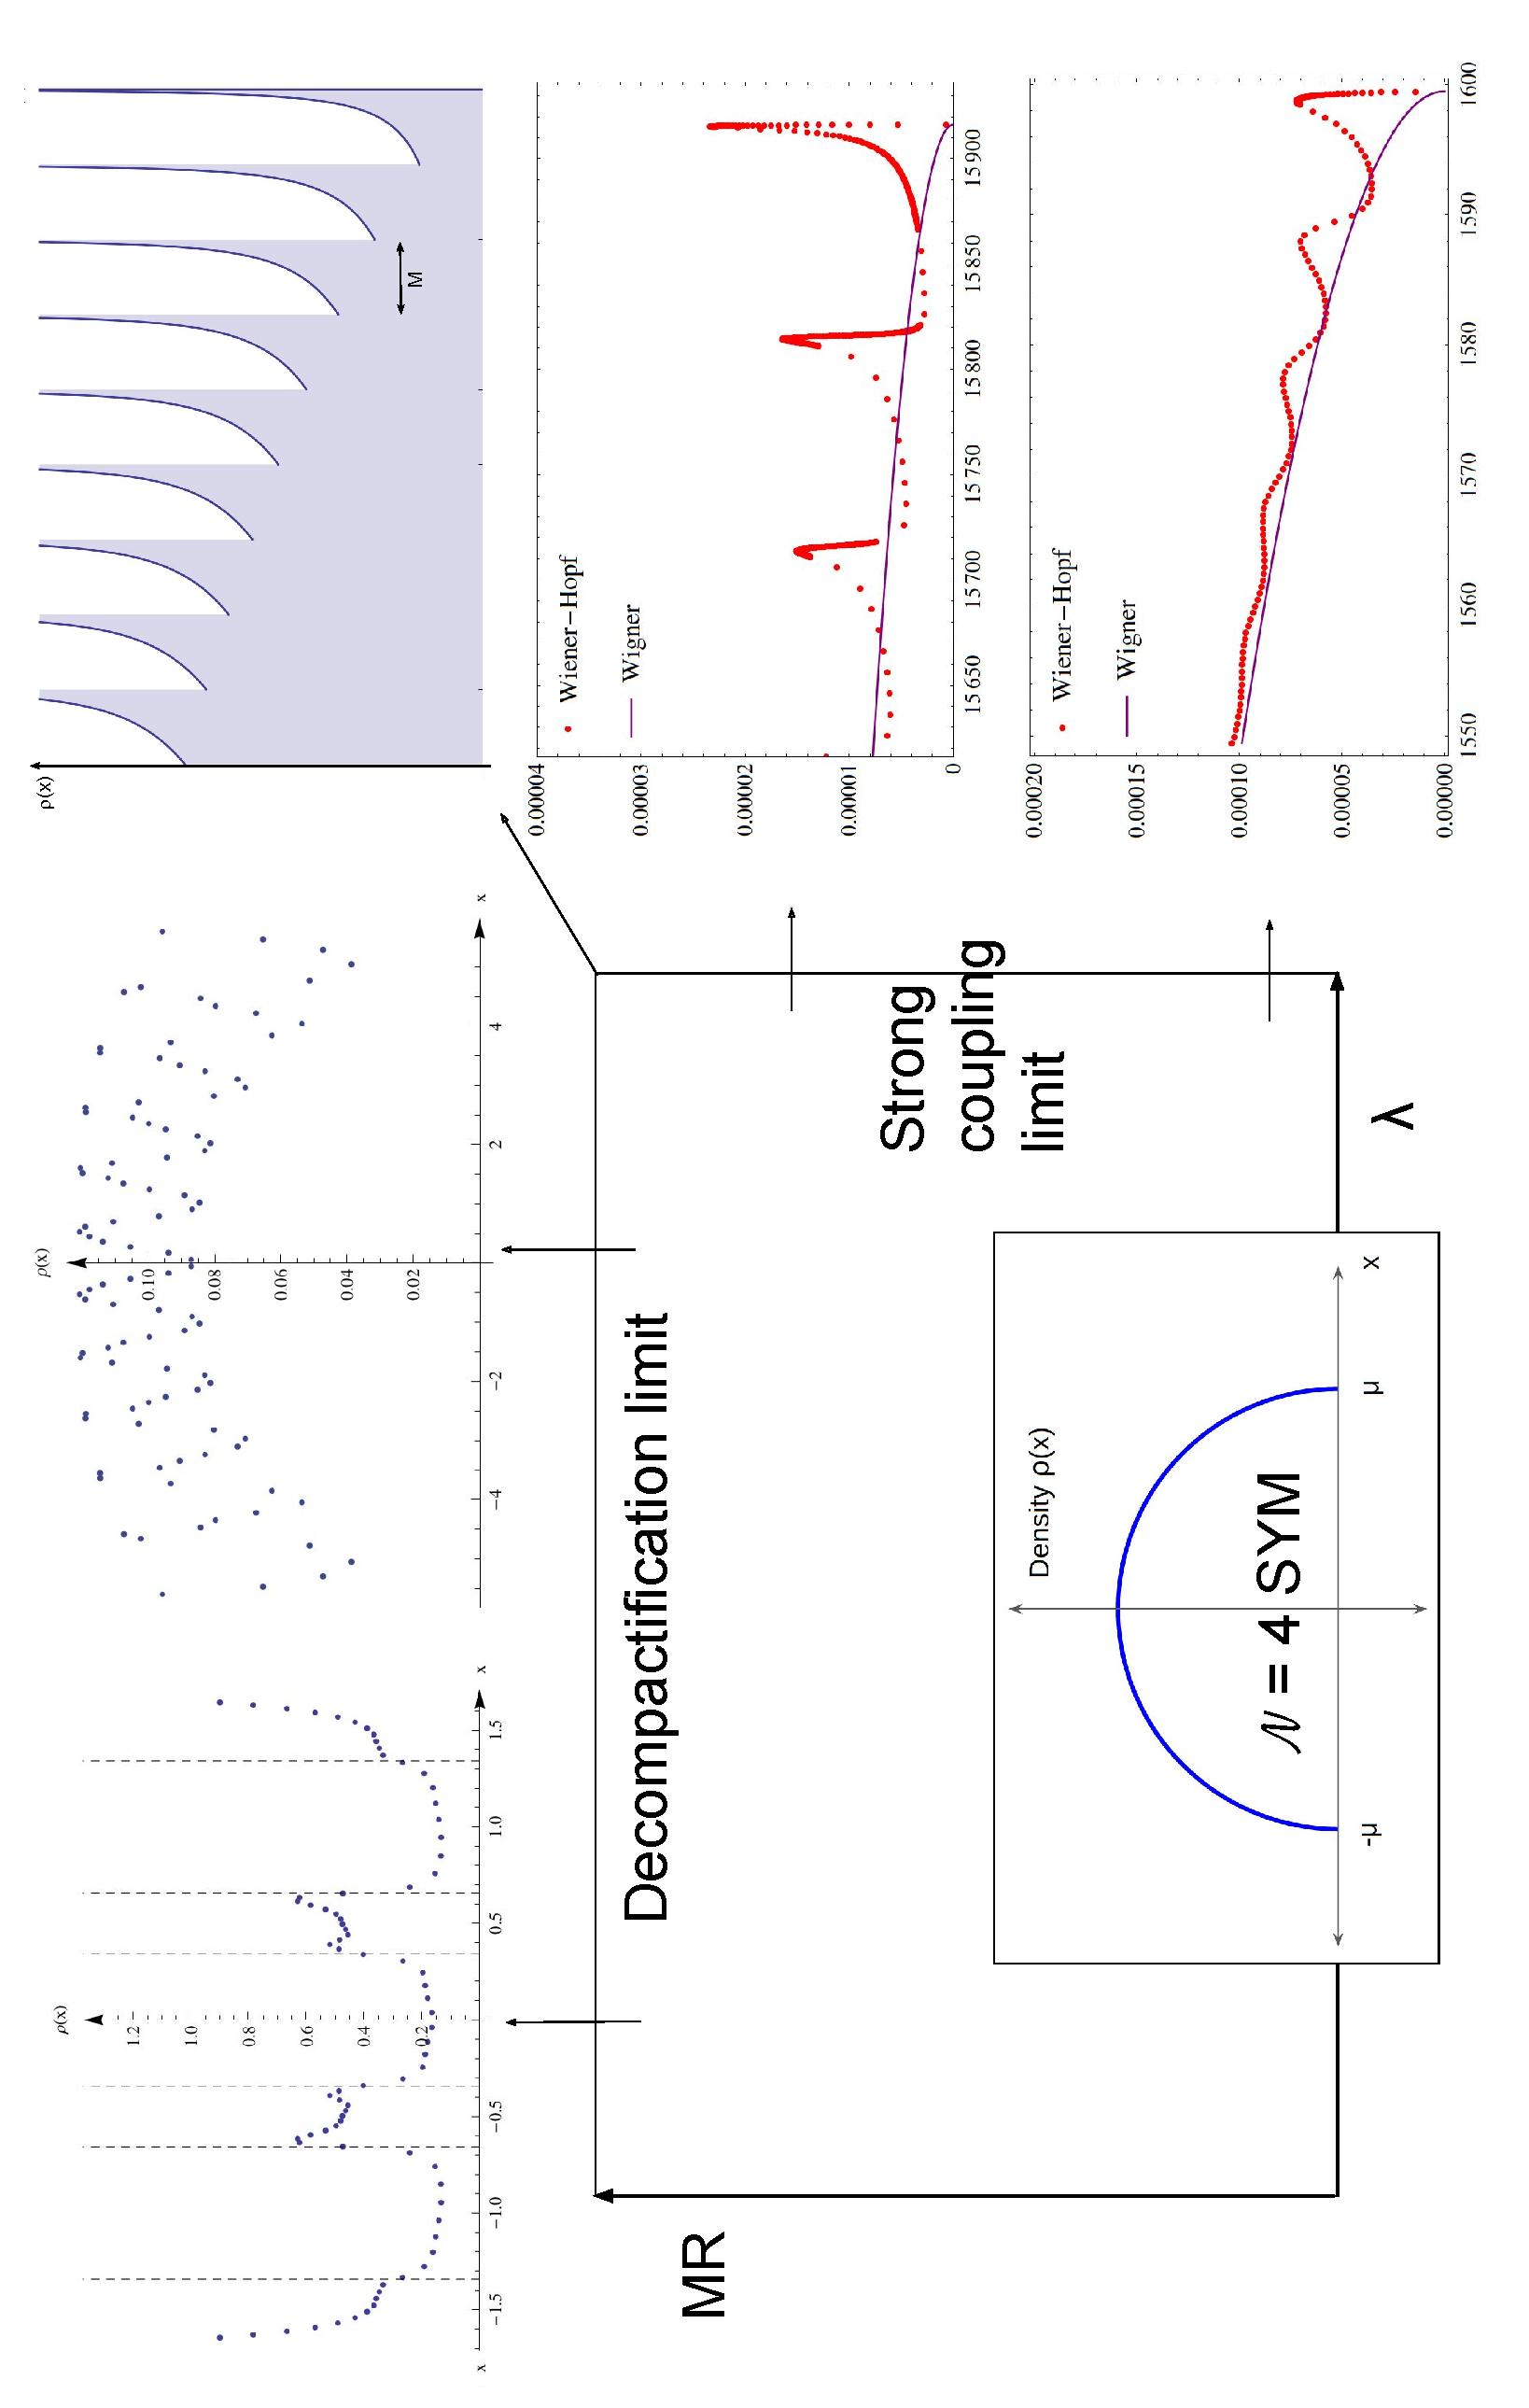
\includegraphics[width=0.9\textwidth]{Images/phaseDiagram.pdf}}
\end{center}
\caption{\label{fig:phaseDiagram} Phase diagram for the partition function of $\mathcal{N}=2^*$ SYM on $S^4$, in the large $N$ limit. 
The plots at the decompactification limit are taken from \cite{Russo:2013qaa}, and the ones at strong coupling limit are from Paper I, where only close to the endpoint is shown and $R=1$.
In the zero mass limit, we have $\mathcal{N}=4$ SYM, where the distribution is the Wigner semicircle for any coupling.}
\end{figure}


Such phase transitions are common among large-$N$ matrix models, 
and have been observed in e.g. ABJM models \cite{Anderson:2014hxa}, 5d $\mathcal{N}=1$ SYM with massive matter multiplets \cite{Nedelin:2015mta}.
In our case, the gauge/string duality in principle gives us an opportunity to understand them from the point of view of gravity.
The physical observables we use to probe the infinite-coupling phase are Wilson loops, the topic of the next chapter.






